% !TeX root = ./00.ppgcc-2020.tex

\section{Implementações Preliminares}\label{sec:resultados}

No desenvolvimento desta pesquisa, uma vez determinado o modelo de operação
distribuída, com processamento nas bordas da rede, algumas experimentações e
algumas ferramentas de teste foram desenvolvidas. Aspectos desses
desenvolvimentos são descritos a seguir.
% obrigado hélio. % :-)

\subsection{Implementação com \python e \kafka}

\notaPA{Inserir Figura para auxiliar na compreensão, principalmente do problema encontrado.}
A primeira implementação e avaliação do \mfog realizada foi construída sobre a
linguagem \python com o sistema de fila de mensagens \kafka e a respectiva
biblioteca de conexão.
A escolha desse conjunto para a implementação ocorreu \hlhl{devido à ampla}
disponibilidade de bibliotecas de aprendizagem de máquina no ecossistema
\python e, à simplicidade geral da linguagem.
Na implementação desenvolvida, o sistema \kafka recebe mensagens e as armazena
em tópicos distribuídos em partições replicadas em nós de um \cluster,
gerenciados por um nó mestre e suportados pelo serviço de gerenciamento de
configuração distribuída \emph{Apache ZooKeeper}.
A aplicação \emph{Python} consome eventos através da interface \emph{Consumer API},
que expõe a distribuição através da associação de um consumidor às partições
mantidas pelo \kafka.

Para essa implementação, havia a hipótese de que a distribuição de
mensagens gerenciada pelo \kafka
se estenderia a processos consumidores, efetivamente distribuindo o volume de
mensagens entre eles igualmente, como ilustrado na Figura \ref{fig:python-kafka}.

\begin{figure}[htb]
    \centerline{
      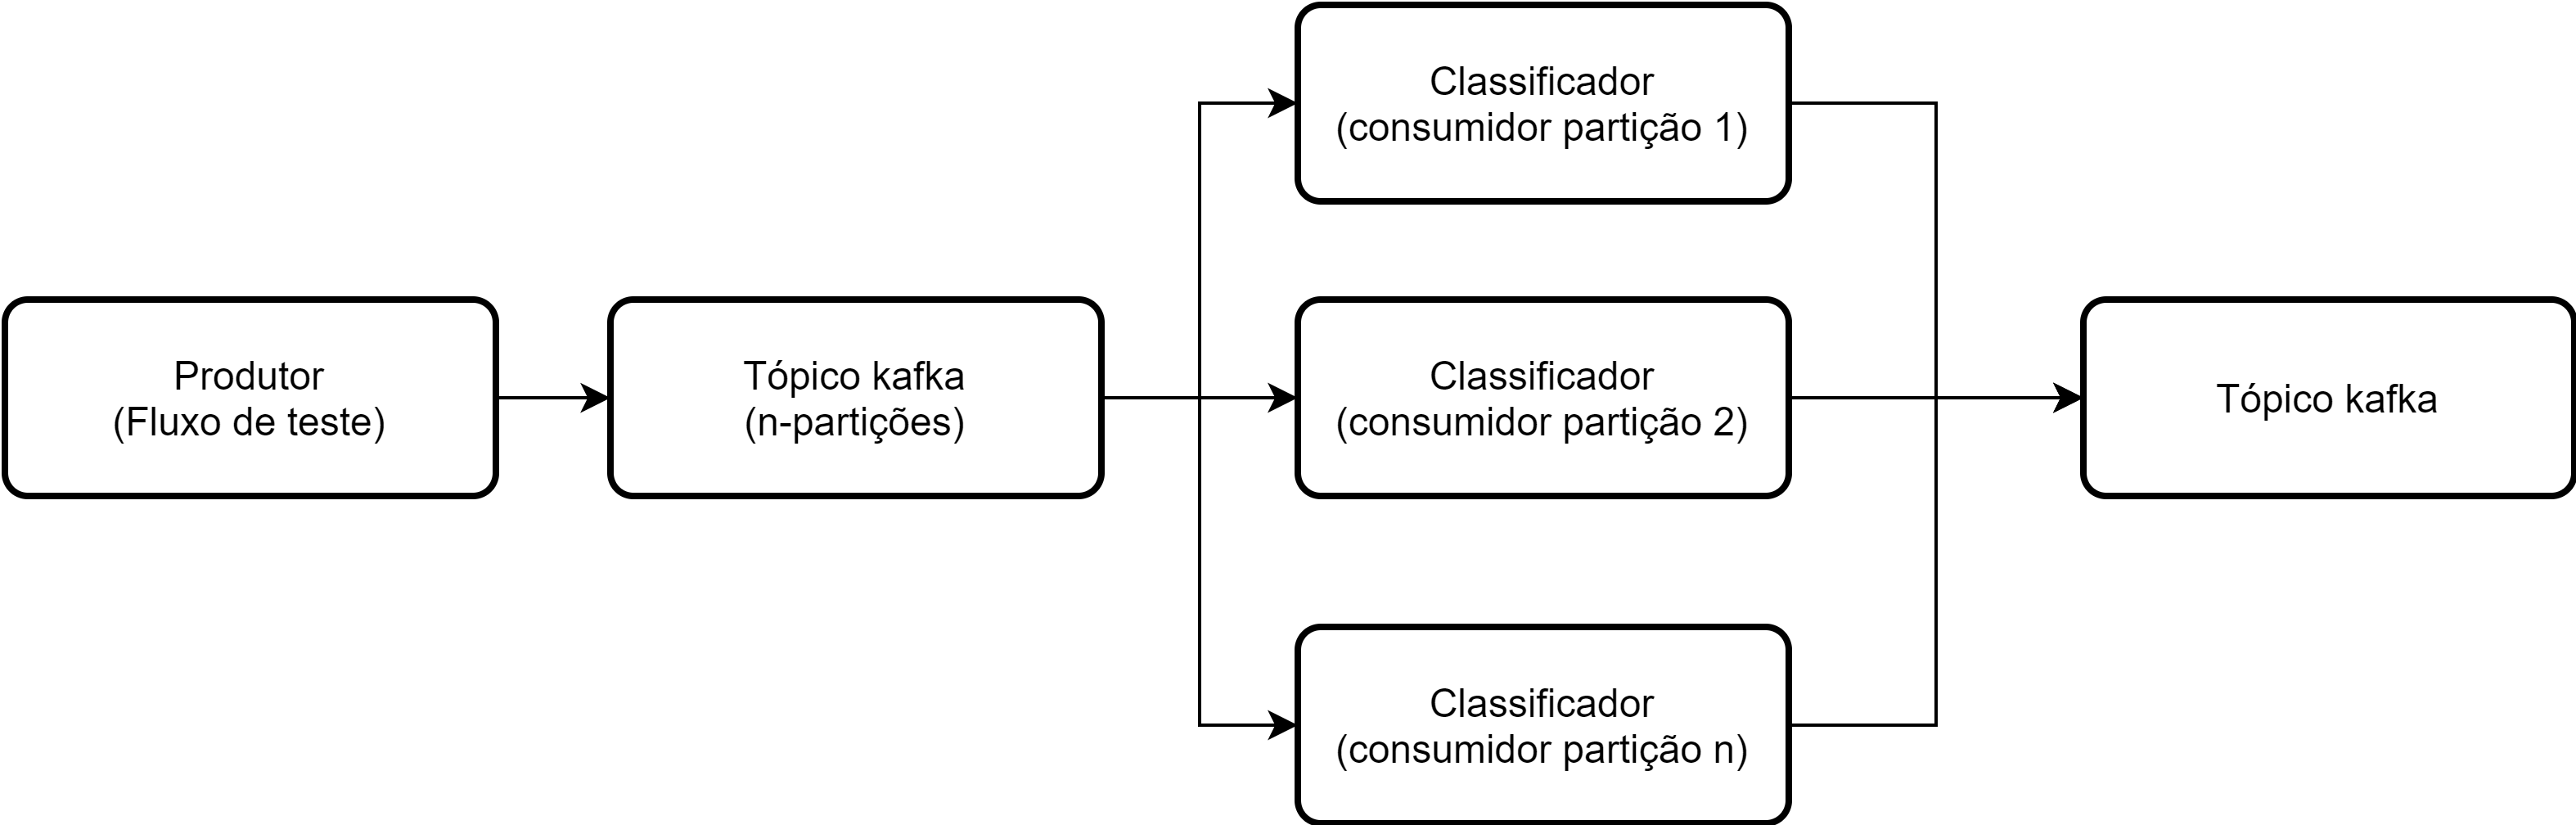
\includegraphics[width=\linewidth,page=1]{figures/python-kafka.png}
    }
    \caption{Hipótese de distribuição de carga com Apache Kafka e Python.}
    \label{fig:python-kafka}
\end{figure}

No entanto, a hipótese foi refutada nos experimentos realizados.
Os experimentos em questão foram compostos de 8 processos consumidores, um
processo produtor, uma instância \kafka com 8 partições em seu tópico principal
e uma instância \emph{Apache ZooKeeper} associada à instância \kafka.
% A hipótese era que, como o número de partições igualava o número de consumidores,
% cada consumidor associaria-se a uma partição, distribuindo os dados igualmente
% entre os consumidores para a paralelização a execução.
A hipótese foi refutada quando observou-se que o número de
mensagens consumidas por um dos $8$ processos representava a maioria (mais de
$80\%$) do volume introduzido no sistema, o restante das mensagens sendo distribuído entre
outros 3 processos e o restante dos processos não recebia nenhuma mensagem.
Portanto, a iniciativa de implementar o algoritmo MINAS em \python com \kafka e
atingir os objetivos de distribuição falhou, o que levou à reconsideração das
plataformas escolhidas.

% TODO: fiz a parte do "figura para auxiliar na compreensão" mas falta a parte do "principalmente do problema encontrado"
% TODO: Rodar o py-kafka-minas no i7, extrair contagem de exemplos por classificador, gerar gráfico de barras disso. (Faço???)

\subsection{Implementação com \flink}

% \nota{citar ferramentas e a escolha só depois do python e kafka}
% \nota{entre flink e spark, outro grupo de pesquisa já está explorando spark}

A segunda alternativa explorada teve por inspiração o trabalho de
\notaPA{Qual seria o outro grupo? Viegas et al. (2019)?}
\citeonline{Viegas2019} e, \hlpa{como outro grupo de pesquisa} já estava explorando
o algoritmo na plataforma \emph{Apache Spark}, a segunda implementação
foi baseada na plataforma \flink.

A plataforma \flink tem modelos de processamento tanto de fluxos como em lotes.
O modelo em lotes é implementado como extensão do modelo de fluxos e, apesar de
não ser foco desse trabalho, mostrou-se útil para a construção da fase de
treinamento \emph{offline} do algoritmo \minas, \hlpa{já que o conjunto consumido por
esse módulo é limitado.}
\notaPA{Não sei se compreendi corretamente. O modelo em lotes é pior, mas pode
ser usado para treinamento offline por trabalhar com conjuntos de dados
menores?}

% Um desafio encontrado durante o desenvolvimento da implementação do \mfog foi a falta
% de bibliotecas na plataforma \flink que disponibilizem versões adaptadas
% à plataforma de algoritmos base para o algoritmo MINAS.
% Em especial, a ausência dos algoritmos \emph{K-means} e \emph{CluStream}
% gerou carga imprevista sobre o processo de desenvolvimento
% resultando no atraso do processo de desenvolvimento.

% Esta implementação segue a arquitetura descrita na \refsec{descricao} e as
% avaliações e resultados esperados descritos neste \refcap{proposta}
% referem-se à implementação do \mfog na plataforma \flink.

Após desenvolvimento e testes em um computador pessoal, o sistema foi testado no
ambiente de testes como descrito na Seção \ref{sec:ambiente}, onde observou-se uma
\notaPA{Definir "enorme"!}
\hlpa{redução enorme} no desempenho que \hlpa{concluiu-se ser causada pelo uso excessivo de
memória pela plataforma \flink}.
\notaPA{Isso provocou uso de swap ou apenas mais acessos? Qual foi o gargalo?}
Com a configuração dos parâmetros de memória do cluster, \hlpa{resultados
\notaPA{Definir "resultados compatíveis com o esperado".}
compatíveis com o esperado} foram obtidos; no entanto, apesar de exemplos de
sucesso na literatura
\cite{lee2017data,Greco2019wearableStream,battulga2020fogguru}, \hlpa{o ambiente de
\notaPA{o código do Apache Flink é aberto?
Esse problema não é apenas falta de liberação de memória?}
testes não permaneceu estável para execução de repetições do experimento,
necessitando reinicializações para que o controlador não ocupasse mais de $1GB$
na segunda execução}, o que \hlpa{degradava imensamente} o desempenho.
\notaPA{O termo "imensamente" é mesmo necessário?}

Em conclusão, apesar de promissora, a plataforma \flink ainda não suportava a
execução em dispositivos computacionais restritos de maneira confiável, sendo a
principal barreira o uso excessivo de memória, comum em plataformas do gênero
\emph{Big Data}.

% 2020-04-27T15:00:32.782 INFO  Classifier Ran baseline in 1408.8210000000001s
% jobmanager.heap.size: 100m
% taskmanager.memory.process.size: 800m
% taskmanager.memory.framework.heap.size: 64m
% taskmanager.memory.flink.size: 400m
% taskmanager.memory.managed.size: 100m
